\section{Problem}

The scheduling of conventional thermal power plants is crucial with the rise of renewable energies.
The Unit Commitment Problem (UCP) introduced later in section \ref{backg:ucp} tackles this problem.
\cite{Banos2011}
Also, it can be used with wind energy and thermal power plants to minimize the cost of incorrect weather predictions.
These approaches are also called risk-based because they model the risk of the weather predictions being wrong.
\cite{Chen2008,Abujarad2017}

The number of deployed smart meters in the European Union was 99 million in 2018.
A study by the European Commission projected the number to reach 123 million by 2020.
\cite{Vlachogiannis2019}
With the increasing number of smart meters, the amount of information about energy consumption is growing.
The data is available with a time resolution that was not yet possible.
Due to the high time resolution in the data produced by the smart meters,
the prediction of future power consumption is possible on a house-to-house basis.
This allows for a much better overall prediction of the power consumption of towns or cities.
\cite{Aiello2016, Basu2013}
It presents the possibility to schedule thermal power plants much more precisely
and with a higher time resolution.

In the future, communities with many private renewable energy sources might rely on distributed energy generation.
Distributed energy generation means that the energy produced by a consumer through their renewable energy sources gets added to the grid if the consumer is currently not using this energy.
Additionally, electric vehicles can be used as energy sources when plugged into a charger.
This gives additional degrees of freedom for energy procurement.
\cite{Aiello2016, Zhang2016}

The actual data to validate the approach in section \ref{validation} is based on the claims above about increased time resolution in the data.
Section \ref{validation:data} explains the details of the data selection.

Figure \ref{figure:problem.sketch} is a sketch of the problem that the work considers.
It shows a town with offices and houses, as well as charging stations for electric vehicles.
There are $4$ power plants around the town that are all connected to it.

\begin{figure}
  \centering
  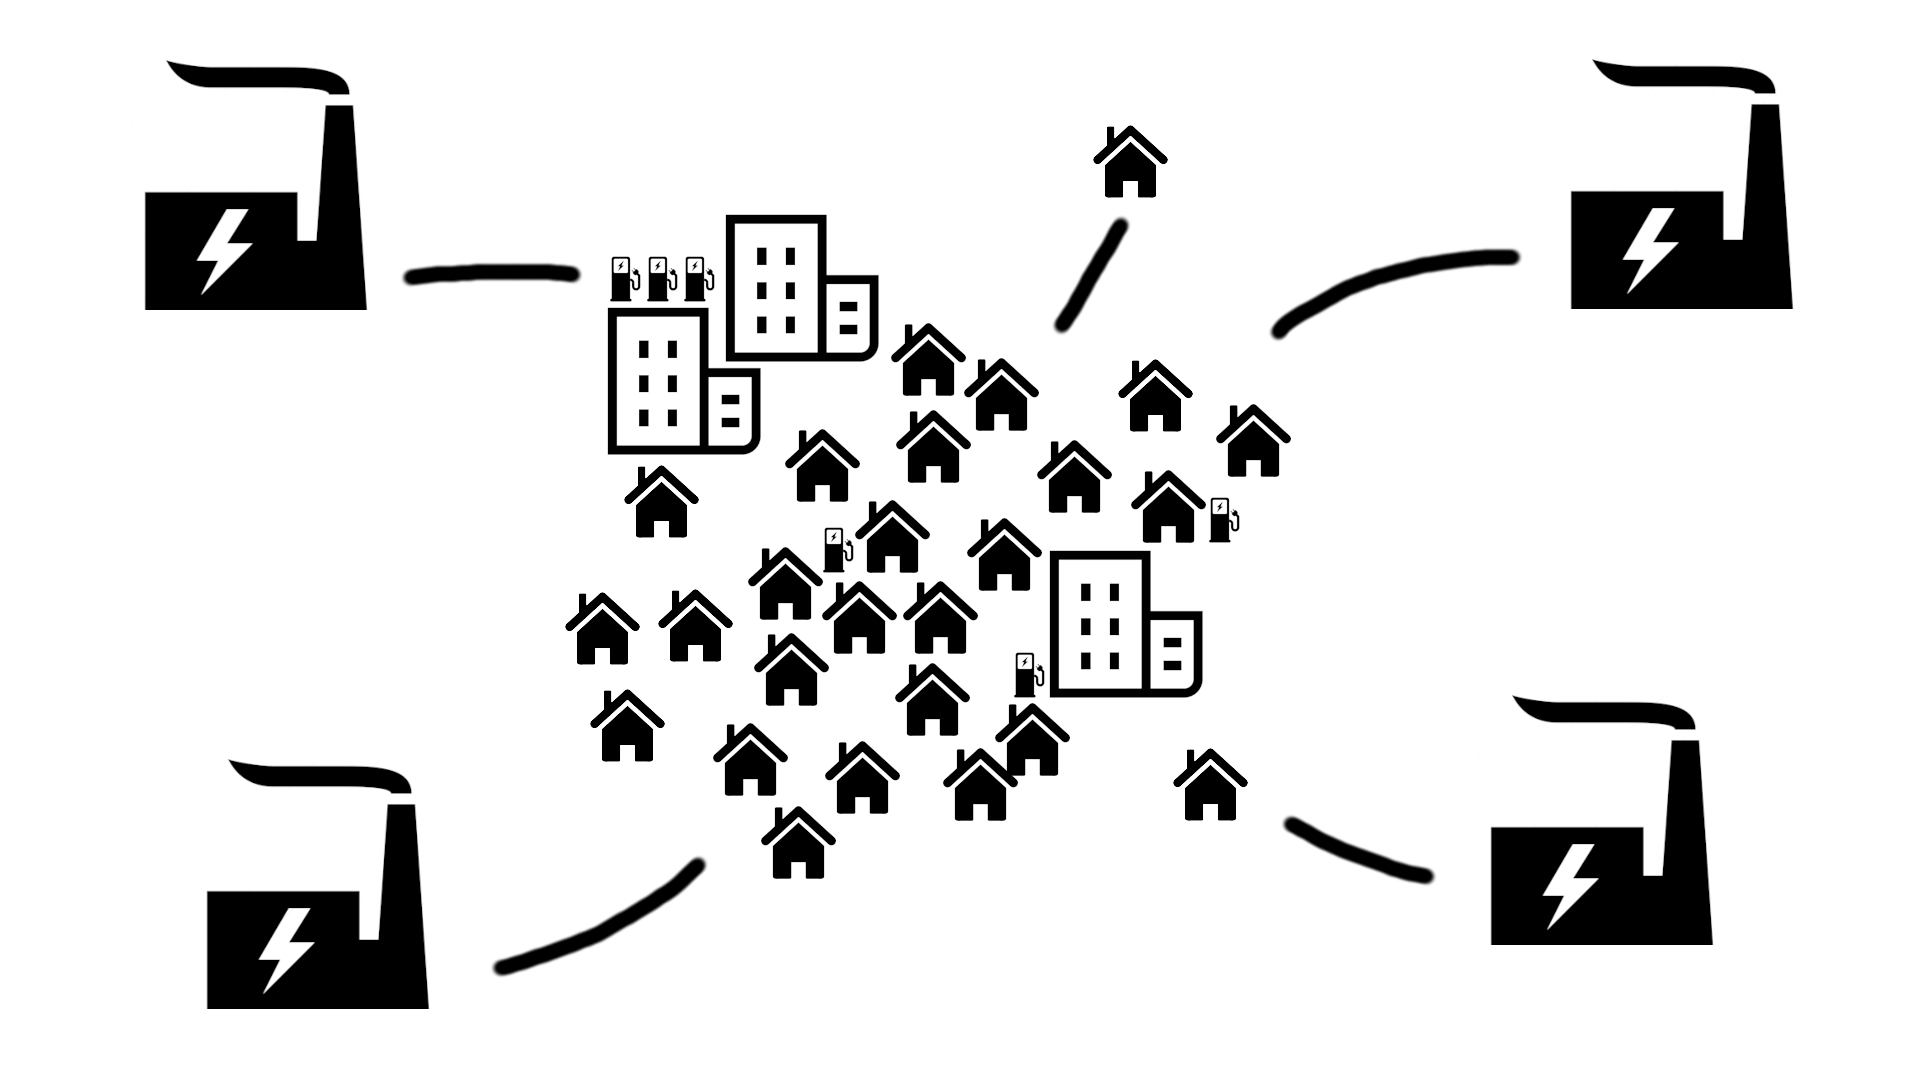
\includegraphics[width=\textwidth]{01_Intro/problem_sketch.png}
  \caption{Sketch of Unit Commitment Problem}
  \label{figure:problem.sketch}
\end{figure}
